\chapter{resultados preliminares}
\section{Disparos dos Elementos Neuronais}
como mostrado na Figura
\subref*{fig:remotojavaspka},
que foi gerada por meio de uma simula��o com 800 MNs do tipo S, 50 do tipo
FR, 50 do tipo FF, 350 CRs e uma corrente de 40 nA injetada no soma de todos
os MNs. Nesse gr�fico, os instantes de disparo dos MNs, representados por 
�ndices, mostram MNs com �ndices menores disparando
depois de outros com �ndices maiores. Como esses �ndices, na simula��o, est�o
relacionados com o tamanho dos MNs, pode-se dizer que ocorreu um certa invers�o
na ordem de recrutamento. 

% TODO put figure in which FR and FF also fire
\begin{figure}[ht!]
    \centering
    \subfloat[][]{
        \label{fig:remotojavaspka}
        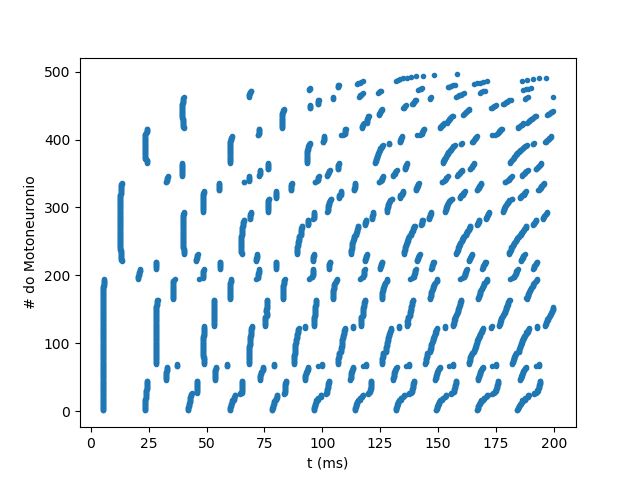
\includegraphics[scale=0.3]{remotojavaspk.png}
    }
    ~ 
    \subfloat[][]{
        \label{fig:remotojavaspkb}
        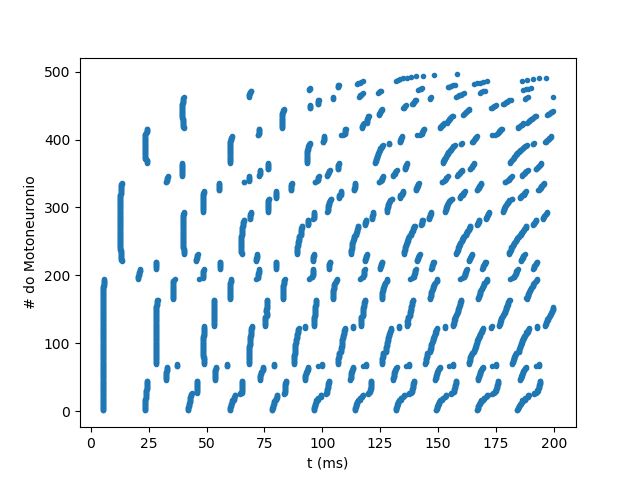
\includegraphics[scale=0.3]{remotojavaspk.png}
    }
    \caption[Momentos de disparo dos somas de todos os motoneur�nios simulados.]{
             Momentos de disparo dos somas de todos os motoneur�nios simulados. O eixo 
             das ordenadas representa o �ndice de cada motoneur�nio em ordem
             crescente de tamanho.
             \subref{fig:remotojavaspkb}.
             \subref{fig:remotojavaspka}.
         }
\end{figure}


\section{Caracter�sticas no Dom�nio da Frequ�ncia}

\section{Desempenho Computacional}
